\documentclass[11pt,a4paper]{article}

\usepackage[utf8]{inputenc}
\usepackage[T1]{fontenc}
\usepackage{lmodern}
\usepackage[margin=0.72in]{geometry}
\usepackage[table]{xcolor}
\usepackage{array}
\usepackage{tabularx}
\usepackage{booktabs}
\usepackage{enumitem}
\usepackage{titlesec}
\usepackage{fancyhdr}
\usepackage{lastpage}
\usepackage{hyperref}
\usepackage{tikz}

\definecolor{TextInk}{HTML}{233142}
\definecolor{HeadingBlue}{HTML}{1D3557}
\definecolor{AccentTeal}{HTML}{2A7F92}
\definecolor{AccentGold}{HTML}{C58B4E}
\definecolor{AccentRed}{HTML}{B85C5A}
\definecolor{RuleGray}{HTML}{D6E0E5}
\definecolor{TableStripe}{HTML}{F3F8FA}
\definecolor{SoftTint}{HTML}{F7F4EE}
\definecolor{SoftBlue}{HTML}{EEF6F8}
\definecolor{SoftGreen}{HTML}{EEF7F0}
\definecolor{SoftRed}{HTML}{FBF0EF}

\hypersetup{
  colorlinks=true,
  linkcolor=HeadingBlue,
  urlcolor=AccentTeal,
  pdftitle={IB Geography SL May 5 Visual Response Workbook},
  pdfauthor={IB Geography SL Preparation}
}

\color{TextInk}
\setlength{\parskip}{0.42em}
\setlength{\parindent}{0pt}
\setlength{\tabcolsep}{5pt}
\renewcommand{\arraystretch}{1.16}
\setlist[itemize]{leftmargin=1.32em,itemsep=3pt,topsep=4pt}
\setlist[enumerate]{leftmargin=1.45em,itemsep=4pt,topsep=5pt}

\newcolumntype{Y}{>{\raggedright\arraybackslash}X}
\newcolumntype{L}[1]{>{\raggedright\arraybackslash}p{#1}}
\newcolumntype{C}[1]{>{\centering\arraybackslash}p{#1}}

\titleformat{\section}
  {\normalfont\Large\sffamily\bfseries\color{HeadingBlue}}
  {}{0pt}{}
  [\vspace{0.08em}{\color{AccentGold}\titlerule[0.8pt]}]
\titleformat{\subsection}
  {\normalfont\large\sffamily\bfseries\color{AccentTeal}}
  {}{0pt}{}

\pagestyle{fancy}
\setlength{\headheight}{14pt}
\fancyhf{}
\fancyhead[L]{\sffamily\color{AccentTeal}May 5 Workbook}
\fancyhead[R]{\sffamily\color{HeadingBlue}IB Geography SL}
\fancyfoot[C]{\sffamily\color{HeadingBlue}\thepage\ of \pageref{LastPage}}
\renewcommand{\headrulewidth}{0.4pt}

\newcommand{\term}[1]{\textcolor{HeadingBlue}{\textbf{#1}}}
\newcommand{\exam}[1]{\textcolor{AccentTeal}{\textbf{#1}}}
\newcommand{\todobox}{\fbox{\rule{0pt}{0.8em}\rule{0.8em}{0pt}}}
\newcommand{\smallline}{\rule{0.96\linewidth}{0.4pt}}
\newcommand{\blankbox}[2]{%
\noindent\fcolorbox{RuleGray}{#1}{%
  \begin{minipage}[t][#2][t]{0.965\textwidth}
  \vspace{0.2em}
  \end{minipage}
}}
\newcommand{\boxnote}[3]{%
\noindent\colorbox{#1}{%
  \begin{minipage}{0.965\textwidth}
  \sffamily
  \textbf{\textcolor{HeadingBlue}{#2}} #3
  \end{minipage}
}}

\begin{document}

\begin{center}
  {\sffamily\bfseries\color{HeadingBlue}\LARGE May 5 Visual-Stimulus Workbook}\\[0.25em]
  {\sffamily\color{AccentTeal}\large Climate Risk, Food / Health Vulnerability, And Policy Evaluation}
\end{center}

\boxnote{SoftBlue}{Strict timing.}{Use \term{15 minutes} for the response set
inside the \term{25 minute} block: \term{3 minutes} source reading,
\term{12 minutes} writing, \term{6 minutes} marking, and \term{4 minutes}
error log.}

\section{Source A: Climate Risk And Human Vulnerability}

The data are illustrative and are designed for visual-stimulus practice. Higher
index values mean a higher level of the indicator.

\rowcolors{2}{TableStripe}{white}
\begin{tabularx}{\textwidth}{L{0.18\textwidth}C{0.14\textwidth}C{0.14\textwidth}C{0.14\textwidth}C{0.15\textwidth}Y}
\toprule
\textbf{Region} & \textbf{Climate-risk index} & \textbf{Food-system vulnerability index} &
\textbf{Health-system stress index} & \textbf{Policy readiness index} &
\textbf{Likely priority} \\
\midrule
Delta Coast & 88 & 72 & 66 & 42 & Flood shelters, drainage, land-use planning \\
Dryland Belt & 76 & 91 & 58 & 35 & Drought planning, water conservation, crop adaptation \\
Heatwave City & 69 & 44 & 84 & 64 & Heat-action plans, shade, healthcare outreach \\
Island Port & 83 & 68 & 61 & 48 & Storm-surge planning, port resilience, import security \\
\bottomrule
\end{tabularx}
\rowcolors{2}{}{}

\subsection{Visual Source A}

Longer bars show higher index values. The four bars for each region show
climate risk, food-system vulnerability, health-system stress, and policy
readiness.

\begin{center}
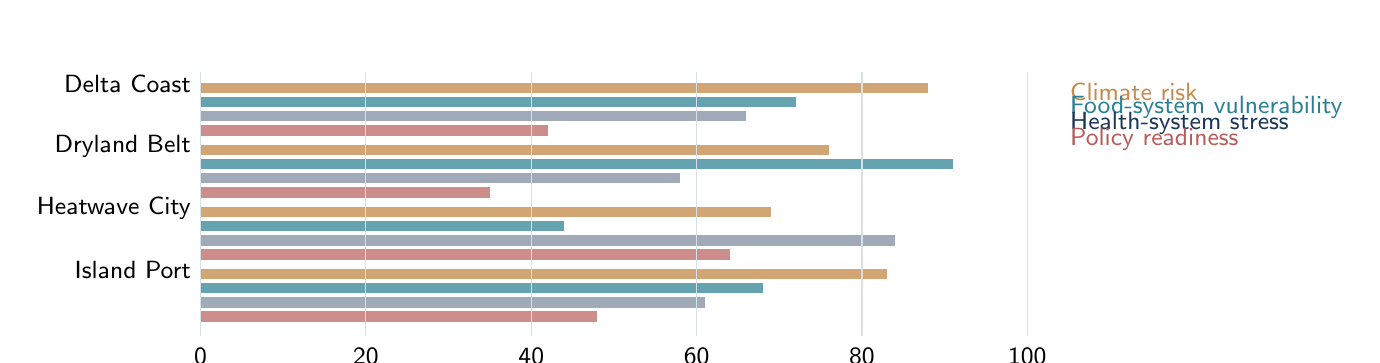
\begin{tikzpicture}[x=0.105cm,y=0.45cm, every node/.style={font=\sffamily\small}]
  \node[anchor=east] at (0,8.1) {Delta Coast};
  \draw[fill=AccentGold!78, draw=none] (0,7.85) rectangle (88,8.15);
  \draw[fill=AccentTeal!72, draw=none] (0,7.45) rectangle (72,7.75);
  \draw[fill=HeadingBlue!42, draw=none] (0,7.05) rectangle (66,7.35);
  \draw[fill=AccentRed!70, draw=none] (0,6.65) rectangle (42,6.95);
  \node[anchor=east] at (0,6.35) {Dryland Belt};
  \draw[fill=AccentGold!78, draw=none] (0,6.10) rectangle (76,6.40);
  \draw[fill=AccentTeal!72, draw=none] (0,5.70) rectangle (91,6.00);
  \draw[fill=HeadingBlue!42, draw=none] (0,5.30) rectangle (58,5.60);
  \draw[fill=AccentRed!70, draw=none] (0,4.90) rectangle (35,5.20);
  \node[anchor=east] at (0,4.60) {Heatwave City};
  \draw[fill=AccentGold!78, draw=none] (0,4.35) rectangle (69,4.65);
  \draw[fill=AccentTeal!72, draw=none] (0,3.95) rectangle (44,4.25);
  \draw[fill=HeadingBlue!42, draw=none] (0,3.55) rectangle (84,3.85);
  \draw[fill=AccentRed!70, draw=none] (0,3.15) rectangle (64,3.45);
  \node[anchor=east] at (0,2.85) {Island Port};
  \draw[fill=AccentGold!78, draw=none] (0,2.60) rectangle (83,2.90);
  \draw[fill=AccentTeal!72, draw=none] (0,2.20) rectangle (68,2.50);
  \draw[fill=HeadingBlue!42, draw=none] (0,1.80) rectangle (61,2.10);
  \draw[fill=AccentRed!70, draw=none] (0,1.40) rectangle (48,1.70);
  \foreach \x in {0,20,40,60,80,100} {
    \draw[RuleGray] (\x,1.0) -- (\x,8.45);
    \node[anchor=north] at (\x,0.92) {\x};
  }
  \node[anchor=west, color=AccentGold] at (104,7.9) {Climate risk};
  \node[anchor=west, color=AccentTeal] at (104,7.45) {Food-system vulnerability};
  \node[anchor=west, color=HeadingBlue] at (104,7.0) {Health-system stress};
  \node[anchor=west, color=AccentRed] at (104,6.55) {Policy readiness};
\end{tikzpicture}
\end{center}

\section{Timed Response Set}

\begin{enumerate}[label=\textbf{\arabic*.}]
  \item Using Source A, \exam{describe} two patterns or contrasts in climate
  risk, food-system vulnerability, health-system stress, or policy readiness.
  \hfill \textbf{[4]}
  \item \exam{Suggest} two reasons why regions with similar climate-risk
  indexes may need different policy responses. \hfill \textbf{[4]}
  \item \exam{State} one policy response shown in Source A and one limitation
  decision-makers should consider when using it. \hfill \textbf{[2]}
\end{enumerate}

\blankbox{white}{10.5cm}

\newpage

\section{Self-Check Before Marking}

\rowcolors{2}{TableStripe}{white}
\begin{tabularx}{\textwidth}{L{0.12\textwidth}Y}
\toprule
\textbf{Done} & \textbf{Check} \\
\midrule
\todobox & I used exact region names and index values in Question 1. \\
\todobox & I described before explaining. \\
\todobox & I used exposure, sensitivity, or capacity to respond in Question 2. \\
\todobox & I named a real policy response from Source A in Question 3. \\
\todobox & I gave a limitation, not just a benefit. \\
\bottomrule
\end{tabularx}
\rowcolors{2}{}{}

\section{Error-Log Sentence}

Complete one sentence.

\boxnote{SoftGreen}{Starter.}{In visual-stimulus questions, I will first
\rule{0.28\linewidth}{0.4pt}, then \rule{0.28\linewidth}{0.4pt}, and I will
evaluate policy by \rule{0.28\linewidth}{0.4pt}.}

\blankbox{white}{3.8cm}

\end{document}
